% Created 2023-01-18 Wed 21:07
% Intended LaTeX compiler: pdflatex
\documentclass[a4paper,12pt,twoside,twocolumn]{article}
\usepackage[utf8]{inputenc}
\usepackage{graphicx}
\usepackage{amsmath}
\usepackage{amssymb}
\usepackage{hyperref}
\usepackage[margin=2cm]{geometry}
\usepackage[sorting=none]{biblatex}

\addbibresource{references/references.bib}
\usepackage{listings}
\usepackage{xcolor}
\definecolor{commentgreen}{RGB}{2,112,10}
\definecolor{eminence}{RGB}{108,48,130}
\definecolor{weborange}{RGB}{255,165,0}
\definecolor{frenchplum}{RGB}{129,20,83}
\definecolor{soft_red}{RGB}{179,20,20}
\lstset{language=Python, frame=tb, tabsize=4, showstringspaces=false, numbers=left, commentstyle=\color{commentgreen}, keywordstyle=\color{eminence}, stringstyle=\color{red}, basicstyle=\small\ttfamily, emph={if,elif,else,def,class}, emphstyle={\color{soft_red}}, escapechar=\&, classoffset=1, otherkeywords={>,<,.,;,-,!,=,~}, morekeywords={>,<,.,;,-,!,=,~}, keywordstyle=\color{weborange}, classoffset=0}
\date{}
\title{Applied machine learning system ELEC0134 22/23 report SN: 17062315}
\hypersetup{pdfborder=0 0 0}

\begin{document}

\setlength\parindent{0pt}
\maketitle

\section{Abstract}
\label{sec:orgea32388}

Artificial Intelligence is evolving faster than ever. One domain in particular, computer vision has benefited from a vast amount of data annotated in the past decades and many recent breakthroughs on the software level.\\

It is now time to develop our own tool built on these discoveries. Its purpose is to tackle challenges in the face recognition area by analysing multiple features of the human face such as its shape, eyes and mouth which are essential to identify individuals and their emotions.\\

To reach this objective, we rely on an important source of annotated data in the form of pictures of celebrities and cartoonish characters.\\

The information from these datasets are then extracted and cleaned before being trained by various algorithms such as Support Vector Machine and Neural Networks which imitate the way human learn in order to make the algorithm able to differentiate individuals.\\

Results are obtained by testing the trained algorithm against a subset of the dataset left aside for this specific purpose.\\

Upon completion of this project, it should be possible to take these proofs of concepts and embed them in more complex systems such as smart cameras and robots which are the most common kind of devices which may benefit from an improved perception.\\

\section{Introduction}
\label{sec:orgc2dc8e6}

Last century, science fiction authors such as Isaac Asimov predicted the rise of intelligent devices \autocite{asimov_akinyemi_2000} \autocite{ai_eco_impact} and now, the dawn of artificial intelligence is upon us. After, the Tay bot \autocite{tay}, it is now the turn of ChatGPT to earn an immense popularity among tech enthusiasts with its ability to provide detailed answers to any question \autocite{chatgpt-detect} \autocite{chatpgt-teach}. And to add to this triumph, Microsoft has shown interest in acquiring OpenAI, the creator of ChatGPT and many other AIs \autocite{microsoft_buy_openai}.\\

But while everyone has their eyes on this new chatbot, a more discrete, albeit, just as interesting revolution, has been ongoing for a few decades already in the computer vision domain.\\

The first visible step toward it was the introduction of captcha \autocite{captcha_original} in 1997. These challenge-response tests quickly became annotation tools channelling the efforts of humans to train artificial intelligences \autocite{captcha_recognition}.\\

Applications are numerous, ranging from biometric tests to disease detection \autocite{cv_cancer} and even robotics with the latest self driving cars \autocite{cv_robotics}.\\

In this report, we shall pay close attention to a specific use case: face recognition. After mentioning the latests relevant breakthroughs, we shall see how we can design softwares able to recognise the gender, emotions, face shape and eye colour of various celebrities and cartoonish characters.\\

\section{Literature survey}
\label{sec:orga176fc9}
Face recognition has been a major topic recently with new algorithms and tools appearing in quick successions as early as last century with, for instance, the creation of Support Vector Machines in 1992, algorithms shining for their adaptability and generalisation ability  \autocite{face_recognition_svm} \autocite{app_svm} or OpenCV created in 2000 and which is a library still widely used in many languages such as C++ and Python \autocite{opencv_face_detect}.\\

Many algorithms were used over the years such as Support Vector Machine and K-nearest neighbour \autocite{recognition_algos}. They all come with their advantages and trade-offs. Convolutional neural networks especially tend to be studied with great attention because of their ability to imitate the human mind which has been AI's goal since its inception \autocite{face_detect_cnn} \autocite{thermal_cnn}.\\

Since various algorithms exist, the main objective nowadays shifted from pure scientific research to engineered solutions to deal with edge cases where computer vision still struggles \autocite{face_reading}.\\

Firstly, faces become harder to analyse with low resolution images and and dim lighting which make data extraction less precise \autocite{gender_classify_facehop}.\\

Moreover noise is more important with data obtained from pictures of people belonging to specific demographic subgroups such as old males, people with darker skin types \autocite{face_detect_disparity} or children which tend to appear as androgynous since gender only becomes more apparent past puberty \autocite{gender_classify_children}.\\

These problems can generally be also explained by biased datasets which contain unbalanced representation of said demographic subgroups \autocite{face_detect_bias}.\\

It is therefore essential to handle data preprocessing with as much care as the analysis itself as we will see in the next sections.\\

\section{Models Description (chart, fig, eq explain/justify)}
\label{sec:org45c1695}
\subsection{Support Vector Machines}
\label{sec:org77cd0f3}

With a linear SVM, we seek w and b such that \(\rho = \frac{2}{\|w\|}\) is maximised and for all \((x_i, y_i), i = 1...n: y_i(w^T x_i + b) \geq 1\).\\

The quadratic operation problem can therefore be reformulated as finding w and b such that: \(\phi(w) = w^Tw\) is minimised for the aforementioned values of \(x\) and \(y\).\\

With that in mind, we just need to solve a dual problem with a Lagrange multiplier \(\alpha_i\) with\\
\(w = \sum \alpha_i y_i x_i\) and \(b = y_k - \sum \alpha_i y_i x_i^Tx_k\) for any \(a_k > 0\). It can be summarised as \(f(x) = \sum \alpha_i y_i x_i^Tx + b\) with every non-zero \(a_i\) indicating the presence of a support vector in the form of \(x_i\).\\

\subsection{Bagging}
\label{sec:orgb4111cf}
\subsection{KNN}
\label{sec:org904e390}
\subsection{Random Forest}
\label{sec:orgfbfecb2}
\section{Implementation (Details. Explain key modules in code)}
\label{sec:orgc64c9e6}
\subsection{Task A1}
\label{sec:orgf7739c5}
\subsection{Task A2}
\label{sec:org6df76a1}
\subsection{Task B1}
\label{sec:org534e6b1}
\subsection{Task B2}
\label{sec:orgda896e5}
\pagebreak\\
\section{Experimental Results and Analysis}
\label{sec:org0d1b554}
\subsection{Task A1}
\label{sec:orga64e71a}
\subsection{Task A2}
\label{sec:org94ebfca}
\subsection{Task B1}
\label{sec:org73a22da}
\subsection{Task B2}
\label{sec:orgba0c434}

\pagebreak\\

\section{Improvements (analysis)}
\label{sec:org1d56b84}

The aforementioned algorithms used for the binary and multiclasses tasks have varying degrees of success.\\

Preprocessing was crucial to avoid noise and underfitting with some algorithms which would have lowered their success below the acceptable threshold.\\

\subsection{Support Vector Machines}
\label{sec:org3c42103}

Regarding Support Vector Machines, the algorithm performed relatively well with task A but could have been improved with a few tricks.\\

\begin{itemize}
\item A better processing for instance entailing standardising inputs properly would be beneficial.\\
\item The same is true about trying different kernels such as the RBF one which perform very well in many situations or even kernels tailored specifically for the task at hand.\\
\item Additionally, fine tuning with weight alteration and modification of the cost function always remains an option as long as it does not lead to overfitting by making the result mostly correlated to a subset of the training data\\
\end{itemize}

\subsection{Convolutional Neural Network}
\label{sec:orgbf8ae9e}

In order to get better results with a CNN, it may be useful to try out the following ideas:\\

\begin{itemize}
\item Try out pre-trained models from the EfficientNet-B which are declined in 8 different versions (from 0 to 7) with incrementally more parameters and a common interface making them easily swappable for quick testing sessions.\\
\item K-fold validation may be particularly useful with various models such as the ones mentioned previously. This strategy relies on splitting the dataset in K groups before selecting all but one for training and using for every iteration a different one for validation, hence getting more consistent results. Note that this represents an example of ensemble learning, a strategy consisting in mixing multiple domains in various ways.\\
\end{itemize}

\section{Conclusion}
\label{sec:org3344feb}

Hence Support Vector Machines and Convolutional Neural Networks are algorithms revered for their high efficiency which was highlighted in those binary and multiclasses tasks related to face recognition.\\

It was essential to pre-process the data with \ldots{}\\



SVMs operate \ldots{} and really shine \ldots{}\\



On the other hand, CNN \ldots{} but are just as efficient \ldots{}\\



We may try next time to mix strategies with different strategies such as K-means clustering which is extremely slow and therefore inefficient but which has the advantage of converging with absolute certitude.\\

Moreover, a more promising alternative would be to try more Deep Learning strategies which imitate the way human learn and work particularly well in tandem with neural networks.\\

Thankfully, the results gathered from the present research should pave the way to better softwares combining them with other strategies such as reinforcement learning in robots and self driving car which could therefore both recognise humans and learn how to drive around them.\\

\begin{center}
\begin{tabular}{lll}
\hline
 &  & \\
\hline
 &  & \\
\hline
\end{tabular}
\end{center}

\pagebreak\\

\begin{figure}[htbp]
\centering
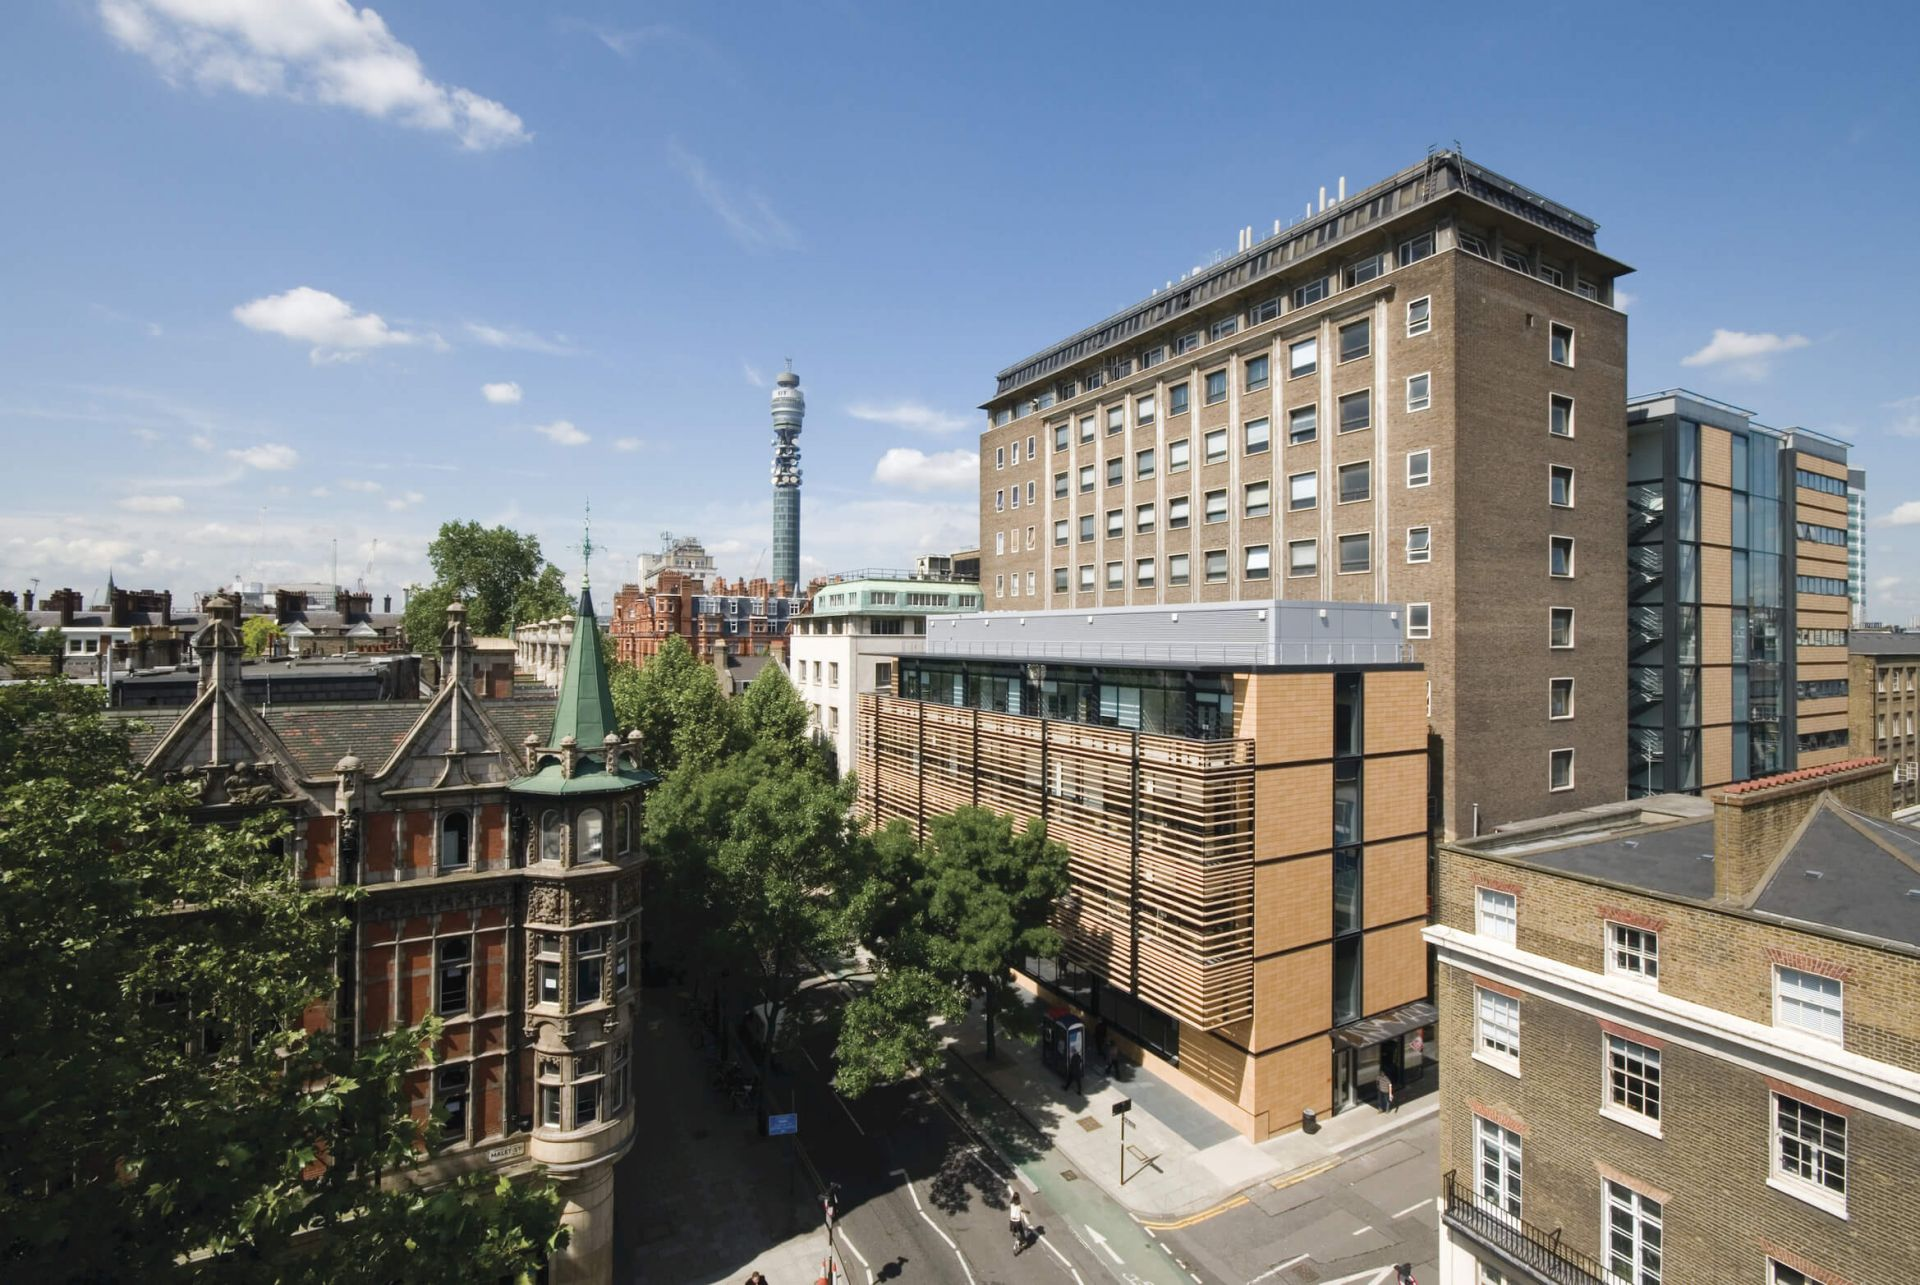
\includegraphics[width=.9\linewidth]{./images/Roberts_building.jpg}
\caption{Caption}
\end{figure}

\lstset{language=Python,label= ,caption= ,captionpos=b,numbers=none}
\begin{lstlisting}
# test
if True == 1 + 1:
    pass

def test

class x
\end{lstlisting}

\vfill \pagebreak \printbibliography\\


\pagebreak\\

\section{Appendix}
\label{sec:org6977499}

This is the output obtained when running the four tasks with 5000 images.\\

\subsection{A1}
\label{sec:org7bbe919}

\begin{verbatim}
: Working on task A1 with label gender from dataset celeba
: Proceeding to get 5000 images including 0.75% for training
: 
: 100% 5000/5000 [01:57<00:00, 42.63it/s]
: Bagging (n=9) 0.5975
: KNN (n=5) 0.7
: Random Forest 0.8275
: SVM (poly) 0.9141666666666667
\end{verbatim}

\subsection{A2}
\label{sec:orgdf9145c}

\begin{verbatim}
: Working on task A2 with label smiling from dataset celeba
: Proceeding to get 5000 images including 0.75% for training
: 
: 100% 5000/5000 [01:57<00:00, 42.66it/s]
: Bagging (n=9) 0.8241666666666667
: KNN (n=7) 0.8558333333333333
: Random Forest 0.8783333333333333
: SVM (poly) 0.8941666666666667
\end{verbatim}

\subsection{B1}
\label{sec:org7a48b7f}

\begin{verbatim}
: Working on task B1 with label face_shape from dataset cartoon_set
: Proceeding to get 5000 images including 0.75% for training
: 
: 100% 5000/5000 [08:58<00:00,  9.29it/s]
: Bagging (n=1) 0.3209028459273798
: KNN (n=8) 0.4867517173699706
: Random Forest 0.6722276741903828
: SVM (poly) 0.7360157016683022
\end{verbatim}

\subsection{B2}
\label{sec:org90a8d3a}

\begin{verbatim}
: Working on task B2 with label eye_color from dataset cartoon_set
: Proceeding to get 5000 images including 0.75% for training
: 
: 100% 5000/5000 [08:59<00:00,  9.27it/s]
: Bagging (n=9) 0.28361138370951916
: KNN (n=9) 0.28949950932286556
: Random Forest 0.34151128557409227
: SVM (poly) 0.3758586849852797
\end{verbatim}
\end{document}